%% FIGURA 1 - Mapa do PJM
\begin{figure}[htb]
	\caption{Região geográfica abrangida pelo PJM dividida em zonas de controle.}
	\begin{center}
	    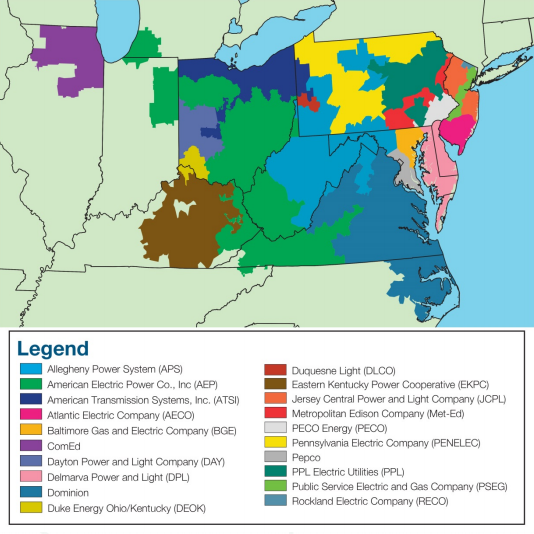
\includegraphics[scale=0.6]{figuras/pjm_map.png}
	\end{center}
    \begin{center}
        \footnotesize {Fonte: \citeonline{pjm2017report}}
    \end{center}
    \label{fig:pjm_map}
\end{figure}

O método utilizado neste projeto pode ser dividido em etapas que serão percorridas sequencialmente. De modo sumário, essas etapas estão listadas abaixo:
\begin{enumerate}
    \item Estudo do funcionamento de modo geral de um mercado livre de energia e a seguir estudo das especifidades do mercado norte-americano PJM;
    \item Seleção dos nós que serão objetos de estudo;
    \item Obtenção e tratamento dos dados dos nós em questão;
    \item Equações de envelhecimento da bateria aplicadas no AMPL;
    \item Análise dos dados obtidos com ferramenta de \textit{business analytics}
\end{enumerate}
---

O método empregado neste projeto consiste essencialmente em:
\begin{itemize}
\item Modelagem e simulação em software de um parque eólico, composto por aerogeradores de velocidade variável, rede coletora e subestação elevadora, semelhante ao esquema da figura abaixo. Sendo cada aerogerador composto por um Gerador de Indução com Rotor Gaiola de Esquilo (\ac{SCIG}), um conversor back-to-back e um filtro RL, conectado à rede coletora através de um transformador elevador de tensão;
\item Simulação de variações nos regimes de vento em um aerogerador e em um parque eólico;
\item Avaliação dos impactos causados na rede elétrica.
\end{itemize}

Vale ressaltar que, para tais simulações, utiliza-se a ferramenta Simulink do software MATLAB.


%% FIGURA 2 - ESQUEMA DE PARQUE EÓLICO
\begin{figure}[htb]
	\caption{Diagrama de modelo de parque eólico.}
	\begin{center}
	    \includegraphics[scale=.6]{figuras/Diagrama_Parque_Eolico/Diagrama_Parque_Eolico.pdf} 
	\end{center}
   \begin{center}
   \footnotesize {Fonte: \citeonline{osetoreletrico2012}}
   \end{center}
    \label{fig:parqueeolico}
\end{figure}


No diagrama da figura~\ref{fig:parqueeolico}, observa-se que o parque eólico esquematizado possui diversos aerogeradores, representados por círculos em preto. Cada um deles, por gerarem energia em baixa tensão (inferior a 1kV), é conectado a um transformador elevador (pela ligação representada na cor lilás) que, em geral, eleva a tensão para cerca de 34,5kV (média tensão). Tais transformadores são por sua vez conectados a uma rede coletora (representada em laranja, na figura), a qual conecta todos os aerogeradores do parque eólico a um barramento de uma subestação elevadora, na qual eleva-se a tensão para a tensão de transmissão (alta tensão) e conexão ao sistema elétrico, usualmente 138 kV ou 230 kV. Na saída desta subestação, encontra-se uma linha de subtransmissão (em verde, na figura), a qual é conectada ao ponto de conexão com a rede elétrica.

Sendo assim, verifica-se a relevância de tal projeto, uma vez que é possível notar que há uma ligação direta entre as variações dos ventos e mudanças no fluxo de potência na rede coletora e também na tensão no ponto de conexão com a rede.


Dessa forma, inicialmente realizou-se um estudo bibliográfico sobre o funcionamento dos aerogeradores de velocidade variável e as diferentes maneiras de controlar o conversor back-to-back. A partir disso, deu-se início à modelagem do controle do aerogerador.

Por conta do link DC entre os dois lados do conversor back-to-back, é possível separar o controle de cada lado. Sendo assim, optou-se por modelar primeiramente o controle do conversor do lado da rede e, após a verificação de seu funcionamento, o controle do conversor do lado do gerador.
Com ambos controles funcionando correto, passa-se à determinação de um modelo de turbina e à simulação de um aerogerador de velocidade variável com variações no regime de vento.

Os passos seguintes consistem na modelagem do parque eólico completo, na simulação de variações no regime de vento e nas análises dos impactos que tais variações tem no ponto de conexão com a rede elétrica.

A descrição detalhada dos cálculos e da modelagem encontram-se nos itens a seguir.




\section{Sistema de controle do aerogerador}
\label{sec:sistcontrol}


Em sistemas eólicos de velocidade variável com gerador de indução com rotor gaiola de esquilo (\ac{SCIG}), é necessário o uso (em cada aerogerador) de um conversor de energia para ajustar a velocidade do gerador de maneira a extrair a máxima potência disponível pelo vento.

Usualmente, o conversor utilizado é do tipo bidirecional back-to-back, por oferecer uma boa proteção à rede elétrica. Ele é basicamente composto por dois conversores de fonte de tensão \ac{VSC} e um capacitor como link DC, conectando ambos os conversores e permitindo o desacoplamento do controle deles.

O controle do conversor do lado da rede (inversor) é responsável pelo ajuste da tensão DC no capacitor e por assegurar a transmissão de potência através do conversor, com controle da troca de potência reativa. Já o controle do conversor do lado do gerador (retificador) é responsável pelo ajuste da velocidade ou do torque do gerador, utilizando um rastreamento do ponto máximo de potência, \ac{MPPT}, para aumentar a eficiência da conversão de energia \cite{wu2011power}. A ação de tais controles no conversor back-to-back ocorre através da geração de sinais de tensão de referência, os quais são modulados por um modulador do tipo \ac{PWM}, gerando pulsos para o chaveamento do conversor de maneira a obter a resposta requerida por seu sistema de controle.


\subsection{Controle do conversor do lado da rede elétrica}

Para o controle do conversor do lado da rede, um método muito utilizado é o de controle vetorial orientado pela tensão na rede (\ac{GVOVC}).

Basicamente, para esse controle faz-se a decomposição da corrente que vai para a rede ($\vec{i_{g}}$) em duas componentes no plano referencial $dq$ síncrono ($i_{dg}$ e $i_{qg}$), então se utiliza $i_{dg}$ para controlar a tensão DC no capacitor, $V_{DC}$ (denominado como $V_{bus}$ na figura \ref{fig:modelo_gridside}), e $i_{qg}$ para controlar a potência reativa do lado da rede ($Q_{g}$), desacoplando o controle para maior desempenho dinâmico.

O sistema do lado da rede pode ser representado pelo modelo da figura \ref{fig:modelo_gridside}. As tensões na rede ($\vec{v_{g}}$) são senoidais com amplitude e frequência constantes; o filtro (por fase) pode ser simplificado por $L_{f}$ (indutivo puro) com uma resistência parasita $R_{f}$; e as tensões no conversor do lado da rede ($\vec{v_{t}}$, medidas nos pontos `a', `b' e `c' da figura \ref{fig:modelo_gridside}) possuem amplitude e frequência variáveis.

%% FIGURA 2 - MODELO SISTEMA LADO DA REDE
\begin{figure}[htb]
	\begin{center}
    \caption{Circuito equivalente do sistema do lado da rede.}
	    \includegraphics[scale=.25]{figuras/Grid_side_system_simplified_model/Grid_side_system_simplified_model.pdf} 
	\end{center}
	\begin{center}
    {\footnotesize Fonte: \citeonline{abad2011doubly}}
    \end{center}
    \label{fig:modelo_gridside}
\end{figure}


Para a implementação do controle \ac{GVOVC}, utiliza-se então o seguinte equacionamento:

- Tensão (Geral):
\begin{equation}
\label{eq:vt_geral}
  \vec{v_{t}} = R_{f}\,\vec{i_{g}} + L_{f}\,\frac{\mathrm{d} \vec{i_g}}{\mathrm{d} t} + \vec{v_{g}}
\
\end{equation}


- Tensões por fase (abc):
\begin{equation}
\label{eq:v_abc}
\left\{\begin{matrix}
   v_{at} = R_{f}\,i_{ag} + L_{f}\,\frac{\mathrm{d} i_{ag}}{\mathrm{d} t} + v_{ag}
\\ v_{bt} = R_{f}\,i_{bg} + L_{f}\,\frac{\mathrm{d} i_{bg}}{\mathrm{d} t} + v_{bg}
\\ v_{ct} = R_{f}\,i_{cg} + L_{f}\,\frac{\mathrm{d} i_{cg}}{\mathrm{d} t} + v_{cg} 
\end{matrix}\right. 
\
\end{equation}


Aplicando a notação de espaço vetorial para as equações de modelagem abc, é possível representar as equações elétricas em componentes $\alpha\beta$:
\begin{equation}
\label{eq:v_alphabeta}
\left\{\begin{matrix}
   v_{\alpha t} = R_{f}\,i_{\alpha g} + L_{f}\,\frac{\mathrm{d} i_{\alpha g}}{\mathrm{d} t} + v_{\alpha g}
\\
   v_{\beta t} = R_{f}\,i_{\beta g} + L_{f}\,\frac{\mathrm{d} i_{\beta g}}{\mathrm{d} t} + v_{\beta g}
\end{matrix}\right.
\
\end{equation}

Na versão compacta referida a um plano estacionário:
\begin{equation}
\label{eq:vt_estac}
  \vec{v_{t}}^{s} = R_{f}\,\vec{i_{g}}^{s} + L_{f}\,\frac{\mathrm{d} \vec{i_g}^{s}}{\mathrm{d} t} + \vec{v_{g}}^{s}
\
\end{equation}

sendo:
\begin{equation}
\label{eq:vt_vg_ig_estac}
\left\{\begin{matrix}
   \vec{v_{t}}^{s} = v_{\alpha t} + j\,v_{\beta t}
\\ 
   \vec{v_{g}}^{s} = v_{\alpha g} + j\,v_{\beta g}
\\ 
   \vec{i_{g}}^{s} = i_{\alpha g} + j\,i_{\beta g}
\end{matrix}\right.
\
\end{equation}


Multiplicando essa versão por $ e^{-j\theta} $ (sendo que $ \theta = \omega_{a}\,t $ é a posição angular do plano rotatório de referência), das expressões $\alpha\beta$ obtém-se as expressões $dq$ (plano referencial rotativo):
\begin{equation}
\label{eq:vt_ref_rot}
  \vec{v_{t}}^{a} = R_{f}\,\vec{i_{g}}^{a} + L_{f}\,\frac{\mathrm{d} \vec{i_g}^{a}}{\mathrm{d} t} + \vec{v_{g}}^{a} + j\,\omega_{a}\,L_{f}\,\vec{i_{g}}^{a}
\end{equation}

Para desacoplar e simplificar o sistema, a velocidade angular síncrona escolhida é $ \omega_{a} = \omega_{s} $ (ou seja, a velocidade angular da tensão na rede). Além disso, alinha-se o eixo $d$ à tensão na rede ($ \vec{v_{g}}^{a} $). Logo, obtém-se que as componentes dq da tensão na saída do conversor do lado da rede são:

\begin{equation}
\label{eq:vdt_ref_rot}
  v_{dt} = R_{f}\,i_{dg} + L_{f}\,\frac{\mathrm{d} i_{dg}}{\mathrm{d} t} + v_{dg} - \omega_{s}\,L_{f}\,i_{qg}
\end{equation}

\begin{equation}
\label{eq:vqt_ref_rot}
  v_{qt} = R_{f}\,i_{qg} + L_{f}\,\frac{\mathrm{d} i_{qg}}{\mathrm{d} t} + v_{qg} + \omega_{s}\,L_{f}\,i_{dg}
\end{equation}

sendo:

\begin{equation}
\left\{\begin{matrix}
   v_{dg} = \left |\vec{v_{g}}^{s}  \right |
\\ 
   v_{qg} = 0
\\ 
   \theta = \theta_{g} = \omega_{s}\,t
\end{matrix}\right.
\
\end{equation}


Portanto, as equações do modelo dq do circuito do lado da rede, no referencial síncrono orientado pela tensão na rede, podem ser escritas da seguinte forma:

\begin{equation}
\frac{\mathrm{d} }{\mathrm{d} t}
\begin{bmatrix}
i_{qg} \\ i_{dg}
\end{bmatrix}
=
\begin{bmatrix}
-R_f/L_f & -\omega_s \\ \omega_s & -R_f/L_f
\end{bmatrix}
\,
\begin{bmatrix}
i_{qg} \\ i_{dg}
\end{bmatrix}
+
\frac{1}{L_f}
\,
\begin{bmatrix}
v_{qt}-v_{qg} \\ v_{dt}-v_{dg}
\end{bmatrix}
\end{equation}

Para realizar o desacoplamento dos eixos $dq$, define-se $ \Delta v_{dg} $ e $ \Delta v_{qg} $ como:

\begin{equation}
\label{eq:delta_vdg_ref_sinc}
  \Delta v_{dg} = v_{dt} - v_{dg} + \omega_s\,L_f\,i_{qg}
\end{equation}

\begin{equation}
\label{eq:delta_vqg_ref_sinc}
  \Delta v_{qg} = v_{qt} - v_{qg} - \omega_s\,L_f\,i_{dg}
\end{equation}


Logo, $ i_{dg} $ e $ i_{qg} $ respondem à $ \Delta v_{dg} $ e $ \Delta v_{qg} $ respectivamente, de acordo com a seguinte função de transferência de 1ª ordem:

\begin{equation}
\label{eq:fctr_Fr}
  F_R(s) = \frac{i_{dg}}{\Delta v_{dg}} = \frac{i_{qg}}{\Delta v_{qg}} = \frac{1/R_f}{(1 + s\tau_f)}
\end{equation}

sendo: $ \tau_f = L_f/R_f $

O alinhamento do eixo $d$ com a tensão da rede, também simplifica o cálculo das potências ativa ($P_g$) e reativa ($Q_g$), de maneira que:

\begin{equation}
\label{eq:Pg}
  P_g = \frac{3}{2}\, v_{dg}\,i_{dg}
\end{equation}

\begin{equation}
\label{eq:Qg}
  Q_g = -\frac{3}{2}\, v_{dg}\,i_{qg}
\end{equation}

Para o controle da potência ativa, controla-se a tensão no link DC ($V_{DC}$). Desta maneira, para o controle de $V_{DC}$ utiliza-se o seguinte equacionamento:

\begin{equation}
\label{eq:Vdc}
  C\,\frac{\mathrm{d} V_{DC}}{\mathrm{d} t} = - i_{dc \rightarrow rede} - i_{dc \rightarrow gerador}
\end{equation}

\begin{equation}
\label{eq:rel_Pg_Vdc}
  P_g = \frac{3}{2}\, v_{dg}\,i_{dg} = V_{DC} \, i_{dc \rightarrow rede}
\end{equation}

Considerando $ i_{dc \rightarrow gerador} $ como uma perturbação e $ v_{dg} \approx V_{DC}/2 $ , obtém-se então que a tensão no link DC responde à corrente $ i_{dg} $ de acordo com a seguinte função de transferência de 1ª ordem:

\begin{equation}
\label{eq:fctr_Gv}
  G_v(s) = \frac{V_{DC}}{i_{dg}} = - \frac{3}{4C}\,\frac{1}{s}\
\end{equation}

Sendo assim, controle do conversor do lado da rede pode ser esquematizado conforme o diagrama de blocos da figura \ref{fig:diag_contr_conv_rede}.


%%% FIGURA 3 !!!!!
\begin{figure}[htb]
	\begin{center}
    \caption{Diagrama de blocos do controle do conversor do lado da rede.}
    \includegraphics[scale=.4]{figuras/Diag_Contr_Lado_Rede/GVOVC_final.pdf} 
	\end{center}
	\begin{center}
    \vspace{-1cm}
    %{\footnotesize Fonte: \citeonline{abad2011doubly}}
    \end{center}

    \label{fig:diag_contr_conv_rede}
\end{figure}


E tais funções de transferência ($ F_R(s) $ e $ G_v(s) $) serão ajustadas para sua implementação de maneira a otimizar a simulação.


%\subsection{Ajuste dos controladores PI do controle do conversor do lado da rede}


%%% Ajuste dos PIs de controle das correntes

Para o sistema de controle, cada conversor \ac{VSC} com modulação \ac{PWM} pode ser representado por uma função de transferência de 1ª ordem do tipo:

\begin{equation}
\label{eq:funcao_pwm}
  G_{d}(s) = \frac{v_{out}}{v_{control}} = \frac{1}{1 + s\,T_a}
\end{equation}

Sendo: $T_a = 1/f_{pwm}$ ($f_{pwm}$: frequência de chaveamento do conversor).

Considerando que $\Delta v_{dg} $ e $ \Delta v_{qg} $ são as tensões de saída ($ v_{out} $) dos controladores PIs das correntes $i_{dg}$ e $i_{qg}$, mas que as tensões que se quer controlar são $  v_{dg}^* $ e $ v_{qg}^* $, tem-se que:

\begin{equation}
\label{eq:fctr_idq_g}
  G_d(s)\,F_R(s) = \frac{1}{(1 + s\,T_a)}\,\frac{1/R_f}{(1 + s\,\tau_f)} = \frac{1/R_f}{(1 + s\,T_a)(1 + s\tau_f)}
\end{equation}

Como $ G_d(s)\,F_R(s) $ equivale a uma função de transferência do tipo $ H_{OL,r}(s) = \frac{K}{(1 + s\,T_\alpha)\,(1 + s\,T_\beta)} $, a partir do método de otimização \textit{Symmetrical Optimum Method} (segundo os estudos de \citeonline{optimummethodPID1999} e  \citeonline{optimumcontroller2005}) obtêm-se:

\begin{eqnarray}
  G_c(s) &=& \frac{Ki}{s} + Kp
  \\
  \left \{ a; Ti; Kp \right \} &=& \left \{\frac{1}{\omega_c\,T_\alpha}; a^2\,T_\alpha; \frac{1}{a\,T_\alpha\,K} \right \}
\end{eqnarray}

Sendo que, para este caso:

\begin{eqnarray}
  K &=& 1/R_f
  \\
  T_\alpha &=& T_a
  \\
  T_\beta &=& \tau_f = L_f/R_f  \,\,\,(pois:\,\,T_\alpha << T_\beta)
\end{eqnarray}

Logo: $\omega_c = \frac{2\pi\,f_{pwm}}{20}$ e $a = \frac{1}{\omega_c\,T_a}$.
E, assim, os parâmetros dos PIs de controle das correntes $i_{dg}$ e $i_{qg}$ passaram a ser dados por:

\begin{eqnarray}
  Kp &=& \frac{\tau_f\,R_f}{a\,T_a}
  \\
  Ti &=& a^2\,T_a
  \\
  Ki &=& Kp/Ti
\end{eqnarray}

\begin{equation}
\label{eq:PI_Corr_Grid}
  G_{c,g}(s) = \frac{Ki}{s} + Kp = \frac{i_{dg}}{v_{dg}} = \frac{i_{qg}}{v_{qg}}
\end{equation}


%%% Ajuste do PI de controle da tensão Vdc

Para o ajuste do PI que controla a tensão $V_{DC}$ através da regulação da corrente $i_{dg}^*$ e do PI que controla a potência reativa $Q_g$, adota-se uma função de transferência de 1ª ordem equivalente a um atraso dada por:

\begin{equation}
\label{eq:funcao_cor_corref}
  H_{eq,r}(s) = \frac{i_{dg}}{i_{dg}^*} = \frac{i_{qg}}{i_{qg}^*} = \frac{1}{1 + s\,T_{eq,r}}
\end{equation}

Adotando-se $T_{eq,r} = t_{s,10}/2,3$, sendo $t_{s,10\%}$ equivalente ao tempo de acomodação de 10\% da resposta a um degrau para a função de transferência que equivale a:

\begin{equation}
\label{eq:tf_cl_inner}
  PI_{corrente-rede}\,G_{d}(s)\,F_R(s) = \left( \frac{Ki}{s} + Kp \right)\,\left(\frac{1}{1 + sT_a} \right)\,\left(\frac{1/R_f}{1 + s\tau_f}\right)
\end{equation}

Admitindo $a = 4$ e considerando a relação expressa na equação \ref{eq:fctr_Gv}, pelo método de otimização \textit{Symmetrical Optimum Method} obtêm-se:

\begin{eqnarray}
  Kp &=& \frac{-(4\,C/3)}{a\,T_{eq,r}}
  \\
  Ti &=& a^2\,T_{eq,r}
  \\
  Ki &=& Kp/Ti
\end{eqnarray}

\begin{equation}
\label{eq:PI_Vdc}
  G_{c,v}(s) = \frac{Ki}{s} + Kp = \frac{i_{dg}^*}{(V_{DC}^*-V_{DC})}
\end{equation}



%%% Ajuste do PI de controle da potência reativa

Semelhantemente, para o ajuste do PI que controla a potência reativa $Q_g$, define-se primeiramente uma função de transferência igual a:

\begin{equation}
\label{eq:tf_cl_inner_Q}
  FT(s) = -(3/2)\,V_{nom}\left(PI_{corrente-rede}\,G_{d}(s)\,F_R(s)\right)
\end{equation}

Para a função $FT(s)$, verifica-se sua resposta a um degrau e realiza-se um ajuste do controlador PI para modelo de planta linear (pela função \textit{pidtune} do MATLAB). Em seguida, aproxima-se $FT(s)$ por uma função de transferência equivalente de 1ª ordem com atraso ($t_{delay}$), através do método \textit{Reaction Curve Method} pela seguinte aproximação:

\begin{equation}
\label{eq:react_curve_Q}
  FG(s) = \frac{\bar{y}(s)}{\bar{c}(s)} \approx \frac{K\,e^{s\,t_{delay}}}{1 + s\,\tau}
\end{equation}

Gera-se, assim, uma constante de tempo ($model.time.constant$) e um ganho ($model.gain$), além do atraso ($t_{delay} = model.time.delay$). Dessa maneira, admitindo-se $a = 3$, tem-se os seguintes parâmetros ajustados para o PI de controle da potência reativa:

\begin{eqnarray}
  tc &=& a\,model.time.constant
  \\
  Kp &=& \frac{model.time.constant}{(model.gain*(tc+model.time.delay))}
  \\
  Ti &=& model.time.constant
  \\
  Ki &=& Kp/Ti
\end{eqnarray}

\begin{equation}
\label{eq:PI_Q}
  G_{c,Q}(s) = \frac{Ki}{s} + Kp = \frac{i_{qg}^*}{(Q_{g}^*-Q_{g})}
\end{equation}




%Process Reaction Curve approach to approximate high-order systems by a first-order-plus-timedelay model using step response data. This model can be used to design a PID controller

% % Controle de Potência Reativa

% Q_ref = (1/3)*Sbase;
% Tf_Q = -Tf_cl_inner*3/2*Vnom;
% S = stepinfo(Tf_Q,'SettlingTimeThreshold',0.1);

% c = pidtune(Tf_Q,'PI');
% Kp_Q = c.Kp;
% Ki_Q = c.Ki;

% %Reaction curve
% [y,t] = step(Tf_Q);
% [model,controller] = ReactionCurve(t,y);

% %direct synthesis method
% a = 3;
% tc = a*model.time_constant;
% Kp_Q = model.time_constant/(model.gain*(tc+model.time_delay));
% Ti_Q = model.time_constant;
% Ki_Q = Kp_Q/Ti_Q;







Dessa maneira, conclui-se os ajustes do sistema de controle do conversor do lado da rede elétrica, passando-se à etapa de testes e do ajuste do controle do conversor do lado do gerador.



\subsection{Controle do conversor do lado do gerador}

Existem diferentes métodos para que seja feito o controle de um gerador elétrico \ac{SCIG}. Entre eles, tem-se o controle (direto ou indireto) orientado pelo fluxo do rotor, pelo fluxo do estator, pelo fluxo no entreferro, ou pelo torque.

O controle orientado pelo fluxo do rotor é o mais popularmente utilizado em sistemas de energia eólica, por conta de sua simplicidade e por ser mais fácil de implementar \cite{wu2011power}.

Essencialmente, faz-se a decomposição da corrente do estator do gerador ($\vec{i_s}$) em duas componentes no plano referencial dq síncrono ($ i_{ds} $ e $ i_{qs} $), então se utiliza $ i_{ds} $ para controlar o fluxo do rotor ($ \vec{\lambda_r} $) e $ i_{qs} $ para controlar o torque eletromagnético do gerador ($ T_e $), desacoplando o controle a fim de alcançar maior desempenho dinâmico \cite{wu2011power}.

Para implementar esse controle, utiliza-se por base o circuito equivalente para um gerador de indução no referencial síncrono (mostrado na figura \ref{fig:modelo_GI_refsincr} a seguir) e o seguinte equacionamento (baseado nos estudos de \citeonline{wu2011power}):

Tensões:

- Tensão no estator:

\begin{equation}
\label{eq:vstator_gi}
 \vec{v_{s}} = R_s\,\vec{i_{s}} + \frac{\mathrm{d} \vec{\lambda_{s}}}{\mathrm{d} t} + j\,\omega_s\,\vec{\lambda_{s}} 
\end{equation}

- Tensão no rotor:

\begin{equation}
\label{eq:vrotor_gi}
 \vec{v_{r}} = R_r\,\vec{i_{r}} + \frac{\mathrm{d} \vec{\lambda_{r}}}{\mathrm{d} t} - j\,(\omega_s - \omega_r)\,\vec{\lambda_{r}} = R_r\,\vec{i_{r}} + \frac{\mathrm{d} \vec{\lambda_{r}}}{\mathrm{d} t} - j\,\omega_{sl}\,\vec{\lambda_{r}}
\end{equation}


Fluxos:

- Fluxo do estator:

\begin{equation}
\label{eq:lambda_s}
 \vec{\lambda_{s}} = (L_{ls} + L_m)\,\vec{i_{s}} + L_m\,\vec{i_{r}} = L_s\,\vec{i_{s}} + L_m\,\vec{i_{r}}
\end{equation}

- Fluxo do rotor:

\begin{equation}
\label{eq:lambda_r}
 \vec{\lambda_{r}} = (L_{lr} + L_m)\,\vec{i_{r}} + L_m\,\vec{i_{s}} = L_r\,\vec{i_{r}} + L_m\,\vec{i_{s}}
\end{equation}


Torque eletromagnético:

\begin{equation}
\label{eq:rel_Torque_mominercia_omegamec}
 J\,\frac{\mathrm{d} \omega_{mec}}{\mathrm{d} t} = T_e - T_m
\end{equation}

\begin{equation}
\label{eq:rel_Torque_flux_corr}
 T_e = \frac{3P}{2}\,\Re(j\,\vec{\lambda_{s}}\,\vec{i_{s}}^{*}) = \frac{-3P}{2}\,\Re(j\,\vec{\lambda_{r}}\,\vec{i_{r}}^{*})
\end{equation}


Sendo:
\\ $ \vec{v_{s}} $ e $ \vec{v_{r}} $ -- as tensões vetoriais do estator e do rotor (referida ao estator), respectivamente, em $[V]$.
\\ $ \vec{i_{s}} $ e $ \vec{i_{r}} $ -- as correntes vetoriais do estator e do rotor (referida ao estator), respectivamente, em $[A]$.
\\ $ \vec{\lambda_{s}} $ e $ \vec{\lambda_{r}} $ -- os fluxos vetoriais do estator e do rotor (referido ao estator), respectivamente, em $[Wb]$.
\\ $ R_s $ e $ R_r $ -- as resistências do estator e do rotor (referida ao estator), respectivamente, em $[\Omega]$.
\\ $ L_{ls} $ e $ L_{lr} $ -- as indutâncias de dispersão do estator e do rotor (referida ao estator), respectivamente, em $[H]$.
\\ $ L_m $ -- a indutância magnetizante do gerador, em $[H]$.
\\ $ L_s $ e $ L_r $ -- as indutâncias próprias do estator e do rotor (referida ao estator), respectivamente, em $[H]$.
\\ $ \omega_{s} $ e $ \omega_{r} $ -- as frequências angulares do estator e do rotor, respectivamente, em $[rad/s]$.
\\ $ \omega_{sl} $ -- a frequência angular de escorregamento (\textit{split}) do gerador, em $[rad/s]$.
\\ $ \omega_{mec} $ -- a velocidade mecânica angular do rotor, $ \omega_{mec} = \omega_{r}/P $, em $[rad/s]$.
\\ $ P $ -- o número de pares de pólos do gerador.
\\ $ J $ -- o momento de inércia do rotor, em $[kgm^2]$.
\\ $ T_e $ -- o torque eletromagnético, em $[N.m]$.
\\ $ T_m $ -- o torque mecânico no eixo do gerador, em $[N.m]$. \\


%%% FIGURA 4 - MODELO GI REF SINCRONO     
\begin{figure}[htb]
	\begin{center}
       \caption{Circuito equivalente de gerador de indução no plano referencial síncrono.}
	    \includegraphics[scale=.25]{figuras/Modelo_GI_refsincrono/Modelo_GI_refsincrono.pdf} 
	\end{center}
    \begin{center}
    {\footnotesize Fonte: \citeonline{wu2011power}}
    \end{center}
	\label{fig:modelo_GI_refsincr}
\end{figure}


A orientação pelo fluxo do rotor ocorre através do alinhamento do eixo $d$ do referencial síncrono com o vetor de fluxo do rotor ($ \vec{\lambda_{r}} $), de maneira que a velocidade rotacional do plano referencial equivale a $ \omega_{s} = 2\,\pi\,f_s $ (sendo $ f_s $ a frequência elétrica do estator), e as componentes $dq$ do fluxo do rotor resultantes sejam:

\begin{equation}
\label{eq:lambda_qr_orientfluxrotor}
  \lambda_{qr} = 0
\end{equation}
\begin{equation}
\label{eq:lambda_dr_orientfluxrotor}
  \lambda_{dr} = \sqrt{(\lambda_{r})^2 - (\lambda_{qr})^2} = \lambda_{r}
\end{equation}

Além disso, o torque eletromagnético do gerador pode ser calculado pela equação:

\begin{equation}
\label{eq:Te_lambda_iqs}
 T_e = K_T\,\lambda_{r}\,i_{qs}
\end{equation}

sendo: $ K_T = 3PL_m/2L_r $

No controle indireto orientado pelo fluxo do rotor, o cálculo do ângulo do fluxo do rotor ($ \theta_f $) é obtido por:

\begin{equation}
\label{eq:theta_f_intomega}
 \theta_f = \int (\omega_r - \omega_{sl})dt
\end{equation}

Sendo $ \omega_r $ a velocidade angular do rotor medida e $ \omega_{sl} $ a frequência de escorregamento calculada.

A partir de manipulações matemáticas das equações anteriores, obtém-se que:

\begin{equation}
\label{eq:lambda_r_is}
\begin{matrix}
  s\,\vec{\lambda_{r}} = -\frac{R_r}{L_r}\,(\vec{\lambda_{r}} - L_m\,\vec{i_{s}}) - j\,\omega_{sl}\,\vec{\lambda_{r}}
\\
  \vec{\lambda_{r}}(1 + \tau_r(s + j\,\omega_{sl})) = L_m\,\vec{i_{s}}
\end{matrix}
\end{equation}

Sendo $ \tau_r = L_r/R_r $ (constante de tempo do rotor).

Decompondo em componentes $dq$, e levando em conta a orientação pelo fluxo, tem-se:

\begin{equation}
\left\{\begin{matrix}
  \lambda_{r}(1 + s\,\tau_r) = L_m\,i_{ds}
\\ 
  \omega_{sl}\,\tau_r\,\lambda_{r} = L_m\,i_{qs}
\end{matrix}\right.
\end{equation}

Logo, a frequência de escorregamento pode ser calculada como:
\begin{equation}
\label{eq:omega_sl}
  \omega_{sl} = \frac{L_m}{\tau_r\,\lambda_r}\,i_{qs}
\end{equation}

De maneira que, nesse tipo de controle (indireto orientado pelo fluxo do rotor), o ângulo do fluxo do rotor $ \theta_f $ para orientação do campo é obtido pela medição da velocidade do rotor $ \omega_r $ e pelo valor de $\omega_{sl}$ calculado, através de um integrador.

Para a obtenção do módulo do fluxo do rotor, tem-se que:

\begin{equation}
\label{eq:lambda_r}
  \lambda_{r} = \frac{L_m}{(1 + s\,\tau_r)}\,i_{ds}
\end{equation}

O valor nominal do módulo do fluxo do rotor é utilizado como referência ($\lambda_r^*$) para o controle. 
E a partir das medições da velocidade do vento ou da velocidade mecânica angular do eixo da turbina, o bloco \ac{MPPT} gera uma velocidade angular de referência $\omega_r^*$. Através dessa referência, adotando-se $T_m = 0$ e aplicando a equação \ref{eq:Te_lambda_iqs} na equação \ref{eq:rel_Torque_mominercia_omegamec}, obtém-se a referência $i_{qs}^*$ pela seguinte função de transferência de 1ª ordem:

\begin{equation}
\label{eq:fctr_omega_iqs}
  G_w(s) = \frac{\omega_r}{i_{qs}^*} = \frac{K_T\,\lambda_r}{J}\,\frac{1}{s}
\end{equation}

Assim, o controle do conversor do lado do gerador pode ser esquematizado conforme o diagrama de blocos da figura \ref{fig:diag_contr_conv_gerador}.


%%% FIGURA 5!!!!!!!!!

\begin{figure}[htb]
	\begin{center}
    \caption{Diagrama de blocos do controle do conversor do lado do gerador.}
    \includegraphics[scale=.4]{figuras/Diag_Contr_Lado_Gerador/Diag_Contr_Lado_Gerador_wref.pdf} 
	\end{center}
    \label{fig:diag_contr_conv_gerador}
\end{figure}



Para o ajuste dos controladores do tipo \ac{PI} que relacionam as componentes $dq$ da tensão e da corrente do estator, é necessário obter as funções de transferência equivalentes. A partir do modelo de gerador de indução e das equações descritas anteriormente, tem-se para o eixo $d$:

\begin{eqnarray}
  v_{ds} &=& R_{s}\,i_{ds} + \frac{\mathrm{d} \lambda_{ds}}{\mathrm{d} t} - \omega_{s}\,\lambda_{qs}
  \\
  v_{ds} &=& R_{s}\,i_{ds} + \frac{\mathrm{d} (L_s\,i_{ds} + L_m\,i_{dr})}{\mathrm{d} t} - \omega_{s}\,(L_s\,i_{qs} + L_m\,i_{qr})
  \\
  v_{ds} &=& R_{s}\,i_{ds} + L_{s}\,\frac{\mathrm{d} i_{ds}}{\mathrm{d} t} + L_{m}\,\frac{\mathrm{d} i_{dr}}{\mathrm{d} t} - \omega_{s}\,L_s\,i_{qs} - \omega_{s}\,L_m\,i_{qr}
  \\
  v_{ds} &=& R_{s}\,i_{ds} + L_{s}\,\frac{\mathrm{d} i_{ds}}{\mathrm{d} t} + L_{m}\,\left(\frac{1}{L_r}\,\frac{\mathrm{d} \lambda_{r}}{\mathrm{d} t} - \frac{L_m}{L_r}\,\frac{\mathrm{d} i_{ds}}{\mathrm{d} t}\right) - \omega_{s}\,L_s\,i_{qs} + \omega_{s}\,\frac{L_m^2}{L_r}\,i_{qs}
  \label{eq:equac_vds}
\end{eqnarray}

Considerando o fluxo do rotor como constante, tem-se que: $ \frac{\mathrm{d} \lambda_{r}}{\mathrm{d} t} \rightarrow 0 $
Portanto,

\begin{equation}
\label{eq:vds}
  v_{ds} = R_{s}\,i_{ds} + \left (L_s - \frac{L_m^2}{L_r} \right)\,\frac{\mathrm{d} i_{ds}}{\mathrm{d} t} - \omega_{s}\,\left (L_s - \frac{L_m^2}{L_r} \right)\,i_{qs}
\end{equation}

Seja $ D_1 = \left (L_s - \frac{L_m^2}{L_r} \right) $, tem-se que:

\begin{equation}
\label{eq:vds}
  v_{ds} = R_{s}\,i_{ds} + D_1\,\frac{\mathrm{d} i_{ds}}{\mathrm{d} t} - \omega_{s}\,D_1\,i_{qs}
\end{equation}


Fazendo o equacionamento para a componente $v_{qs}$, obtém-se:

\begin{eqnarray}
\label{eq:equac_vqs}
  v_{qs} &=& R_{s}\,i_{qs} + \frac{\mathrm{d} \lambda_{qs}}{\mathrm{d} t} + \omega_{s}\,\lambda_{ds}
  \\
  v_{qs} &=& R_{s}\,i_{qs} + \frac{\mathrm{d} (L_s\,i_{qs} + L_m\,i_{qr})}{\mathrm{d} t} + \omega_{s}\,(L_s\,i_{ds} + L_m\,i_{dr})
  \\
  v_{qs} &=& R_{s}\,i_{qs} + L_{s}\,\frac{\mathrm{d} i_{qs}}{\mathrm{d} t} + L_{m}\,\frac{\mathrm{d} i_{qr}}{\mathrm{d} t} + \omega_{s}\,L_s\,i_{ds} + \omega_{s}\,L_m\,i_{dr}
  \\
  v_{qs} &=& R_{s}\,i_{qs} + L_{s}\,\frac{\mathrm{d} i_{qs}}{\mathrm{d} t} + L_{m}\,\left(-\frac{L_m}{L_r}\,\frac{\mathrm{d} i_{qs}}{\mathrm{d} t}\right) + \omega_{s}\,L_s\,i_{ds} + \omega_{s}\,L_m\,\left(\frac{\lambda_r}{L_r} - \frac{L_m}{L_r}\,i_{ds}\right)
  \\
  v_{qs} &=& R_{s}\,i_{qs} + \left (L_s - \frac{L_m^2}{L_r} \right)\,\frac{\mathrm{d} i_{qs}}{\mathrm{d} t} + \omega_{s}\,\left (L_s - \frac{L_m^2}{L_r} \right)\,i_{ds} + \omega_{s}\,\frac{L_m}{L_r}\,\lambda_r
\end{eqnarray}


Considerando $\left(\omega_{s}\,\frac{L_m}{L_r}\,\lambda_r \right)$ como uma perturbação, para obter um controle simplificado de 1ª ordem é necessário desprezar sua influência no cálculo da componente q da tensão no estator do gerador. Logo, tem-se:

\begin{equation}
\label{eq:vqs}
  v_{qs} = R_{s}\,i_{qs} + D_1\,\frac{\mathrm{d} i_{qs}}{\mathrm{d} t} + \omega_{s}\,D_1\,i_{ds}
\end{equation}

Portanto, as equações do modelo $dq$ do gerador de indução \ac{SCIG}, no referencial síncrono, podem ser escritas da seguinte forma:

\begin{equation}
\frac{\mathrm{d} }{\mathrm{d} t}
\begin{bmatrix}
i_{ds} \\ i_{qs}
\end{bmatrix}
=
\begin{bmatrix}
-R_s/D_1 & \omega_s \\ -\omega_s & -R_s/D_1
\end{bmatrix}
\,
\begin{bmatrix}
i_{ds} \\ i_{qs}
\end{bmatrix}
+
\frac{1}{D_1}
\,
\begin{bmatrix}
v_{ds} \\ v_{qs}
\end{bmatrix}
\end{equation}


Para realizar o desacoplamento dos eixos $dq$, define-se $\Delta v_{ds}$ e $\Delta v_{qs}$ como:

\begin{equation}
\label{eq:delta_vds}
  \Delta v_{ds} = v_{ds} + \omega_s\,D_1\,i_{qs}
\end{equation}

\begin{equation}
\label{eq:delta_vqs}
  \Delta v_{qs} = v_{qs} - \omega_s\,D_1\,i_{ds}
\end{equation}


Logo, $ i_{ds} $ e $ i_{qs} $ respondem à $ \Delta v_{ds} $ e $ \Delta v_{qs} $ respectivamente, de acordo com a seguinte função de transferência de 1ª ordem:

\begin{equation}
\label{eq:fctr_F}
  F(s) = \frac{i_{ds}}{\Delta v_{ds}} = \frac{i_{qs}}{\Delta v_{qs}} = \frac{1}{(R_s + sD_1)}  = \frac{1/R_s}{(1 + s\tau_s)}
\end{equation}

sendo: $ \tau_s = D_1/R_s = \left (L_s - \frac{L_m^2}{L_r} \right)/R_s  $


As funções de transferência $G_w(s)$ e $F(s)$ serão ajustadas para sua implementação de maneira a otimizar a simulação.


%%% Ajuste dos PIs de controle das correntes

Conforme visto no equacionamento do ajuste e otimização dos controladores PI do sistema de controle do lado da rede, cada conversor \ac{VSC} com modulação \ac{PWM} pode ser representado por uma função de transferência de 1ª ordem do tipo:

\begin{equation}
  G_{d}(s) = \frac{v_{out}}{v_{control}} = \frac{1}{1 + s\,T_a}
\end{equation}

Sendo: $T_a = 1/f_{pwm}$ ($f_{pwm}$: frequência de chaveamento do conversor).

Considerando que $\Delta v_{ds} $ e $ \Delta v_{qs} $ são as tensões de saída ($ v_{out} $) dos controladores PIs das correntes $i_{ds}$ e $i_{qs}$ anteriormente regulados, mas que as tensões que se quer controlar são $  v_{ds}^* $ e $ v_{qs}^* $, tem-se que:

\begin{equation}
\label{eq:fctr_idq_s}
  G_{d}(s)\,F(s) = \frac{1}{(1 + s\,T_a)}\,\frac{1/R_s}{(1 + s\,\tau_s)}
\end{equation}

Como $ G_{d}(s)\,F(s) $ equivale a uma função de transferência do tipo $ H_{OL}(s) = \frac{K}{(1 + s\,T_\alpha)\,(1 + s\,T_\beta)} $, a partir do método de otimização \textit{Symmetrical Optimum Method} (segundo os estudos de \citeonline{optimummethodPID1999} e  \citeonline{optimumcontroller2005}) obtêm-se:

\begin{eqnarray}
  G_c(s) &=& \frac{Ki}{s} + Kp
 \\
  \left \{ a; Ti; Kp \right \} &=& \left \{\frac{1}{\omega_c\,T_\alpha}; a^2\,T_\alpha; \frac{1}{a\,T_\alpha\,K} \right \}
\end{eqnarray}

Sendo que, para este caso:

\begin{eqnarray}
  K &=& 1/R_s
  \\
  T_\alpha &=& T_a = 1/1800
  \\
  T_\beta &=& \tau_s = \sigma\,L_s/R_s  \,\,\,(pois:\,\,T_\alpha << T_\beta)
\end{eqnarray}

Logo: $\omega_c = \frac{2\pi\,f_{pwm}}{20}$ e $a = \frac{1}{\omega_c\,T_a}$.
E, assim, os parâmetros dos PIs de controle das correntes $i_{ds}$ e $i_{qs}$ passaram a ser dados por:

\begin{eqnarray}
  Kp &=& \frac{\tau_s\,R_s}{a\,T_a}
  \\
  Ti &=& a^2\,T_a
  \\
  Ki &=& Kp/Ti
\end{eqnarray}

\begin{equation}
\label{eq:PI_Corr_Gerador}
  G_{c,r}(s) = \frac{Ki}{s} + Kp = \frac{i_{ds}}{v_{ds}} = \frac{i_{qs}}{v_{qs}}
\end{equation}

%%% Ajuste do PI de controle do fluxo do rotor

Para o ajuste do PI que controla o fluxo do rotor $\lambda_{r}$ através da regulação da corrente $i_{ds}^*$ e do PI que controla a velocidade angular do rotor do gerador $\omega_r$, adota-se uma função de transferência de 1ª ordem equivalente a um atraso dada por:

\begin{equation}
\label{eq:funcao_cor_corref_ger}
  H_{eq,r}(s) = \frac{i_{ds}}{i_{ds}^*} = \frac{i_{qs}}{i_{qs}^*} = \frac{1}{1 + s\,T_{eq,rotor}}
\end{equation}

Adotando-se $T_{eq,rotor} = t_{s,10}/2,3$, sendo $t_{s,10\%}$ equivalente ao tempo de acomodação de 10\% da resposta a um degrau para a função de transferência que equivale a:

\begin{equation}
\label{eq:tf_cl_inner_ger}
  PI_{corrente-gerador}\,G_{d}(s)\,F_R(s) = \left( \frac{Ki}{s} + Kp \right)\,\left(\frac{1}{1 + sT_a} \right)\,\left(\frac{1/R_s}{1 + s\tau_s}\right)
\end{equation}

Admitindo $a = 4$ e considerando a relação expressa na equação \ref{eq:lambda_r}, pelo método de otimização \textit{Symmetrical Optimum Method} obtêm-se:

\begin{eqnarray}
  Kp &=& \frac{(\tau_r/Lm)}{a\,T_{eq,rotor}}
  \\
  Ti &=& a^2\,T_{eq,rotor}
  \\
  Ki &=& Kp/Ti
\end{eqnarray}

\begin{equation}
\label{eq:PI_fluxo_rotor}
  G_{c,flux}(s) = \frac{Ki}{s} + Kp = \frac{i_{ds}^*}{(\lambda_{r}^*-\lambda_{r})}
\end{equation}


%%% Ajuste do PI de controle de velocidade
Semelhantemente, para o ajuste do PI que controla a velocidade angular do rotor do gerador $\omega_r$, dado um $\omega_r^*$ (de referência) vindo do bloco \ac{MPPT}, considerando as equações \ref{eq:rel_Torque_mominercia_omegamec} e \ref{eq:Te_lambda_iqs}, além da função de transferência expressa na equação \ref{eq:fctr_omega_iqs}, tem-se que:

\begin{eqnarray}
  Kp &=& \frac{(K_T\,\lambda_r^*/J)}{a\,T_{eq,rotor}}
  \\
  Ti &=& a^2\,T_{eq,rotor}
  \\
  Ki &=& Kp/Ti
\end{eqnarray}

\begin{equation}
\label{eq:PI_velocidade}
  G_{c,w}(s) = \frac{Ki}{s} + Kp = \frac{i_{qs}^*}{(\omega_r^*-\omega_r)}
\end{equation}


Dessa maneira, conclui-se os ajustes do sistema de controle do conversor do lado do gerador, passando-se à etapa de testes.



